%----------------------------------------------------------------------------------------

\documentclass{elsarticle}

\usepackage{amsmath}
\usepackage{bm}
\usepackage{subcaption}
\usepackage{booktabs} % Horizontal rules in tables
\usepackage{enumitem} % Customized lists
\usepackage{graphicx} 
\usepackage{natbib}%[2010/09/13]
\usepackage{changepage}
\usepackage{tikz} 

%%%%%%%%%%%% new commands

\newcommand{\SN}{S$_N$}
\renewcommand{\vec}[1]{\bm{#1}} %vector is bold italic
\newcommand{\vd}{\bm{\cdot}} % slightly bold vector dot
\newcommand{\ud}{\mathop{}\!\mathrm{d}} % upright derivative symbol
%  new definitions
\newcommand{\bs}[1]{\mathbf{#1}}
\renewcommand{\div}{\bs{\nabla}\! \cdot \!}
\newcommand{\grad}{\bs{\nabla}}
% extra space
\newcommand{\qq}{\quad\quad}
% common reference commands
\newcommand{\eqt}[1]{Eq.~(\ref{#1})}                     % equation
\newcommand{\eqts}[2]{Eqs.~(\ref{#1})~and~(\ref{#2})}    % equation
\newcommand{\eqtss}[2]{Eqs.~(\ref{#1})-(\ref{#2})}       % equation
\newcommand{\fig}[1]{Fig.~\ref{#1}}                      % figure
\newcommand{\figs}[2]{Figs.~\ref{#1}~and~\ref{#2}}		% two figures
\newcommand{\figss}[2]{Figs.~\ref{#1}~-~\ref{#2}}			% multiple figures
\newcommand{\tbl}[1]{Table~\ref{#1}}                     % table
\newcommand{\sct}[1]{Section~\ref{#1}}                   % section
\newcommand{\app}[1]{Appendix~\ref{#1}}                  % appendix

\newcommand{\keff}{k_\textit{eff}}

\newcommand{\be}{\begin{equation}}
\newcommand{\ee}{\end{equation}}
\newcommand{\vn}{\vec{n}}
\newcommand{\vel}{\vec{\mathrm{v}}}
\newcommand{\adj}{\Phi^\dagger_0}
\newcommand{\norm}[1]{\left\lVert#1\right\rVert_{L^2}}

\definecolor{britishracinggreen}{rgb}{0.0, 0.26, 0.15}
\newcommand{\tcr}[1]{\textcolor{red}{#1}}
\newcommand{\tcb}[1]{\textcolor{blue}{#1}}
\newcommand{\tcm}[1]{\textcolor{magenta}{#1}}
\newcommand{\tcp}[1]{\textcolor{violet}{#1}}
\newcommand{\tcg}[1]{\textcolor{britishracinggreen}{#1}}

% tikz stuff
\usetikzlibrary{shapes,arrows,positioning}
\pgfdeclarelayer{background}
\pgfdeclarelayer{foreground}
\pgfsetlayers{background,main,foreground}
\tikzstyle{redblock}=[rectangle, draw, align=center, top color=red!25, bottom color=red!75,  minimum width=10mm, minimum height=10mm,]
\tikzstyle{blueblock}=[rectangle,draw, align=center, top color=blue!25, bottom color=blue!75,  minimum width=10mm, minimum height=10mm]
\tikzstyle{purpleblock}=[rectangle,  draw, align=center, top color=purple!25, bottom color=purple!75, minimum width=10mm, minimum height=10mm]
\tikzstyle{orangeblock}=[rectangle, draw, align=center, top color=orange!25, bottom color=orange!75,  minimum width=10mm, minimum height=10mm]
\tikzstyle{greendiamond}=[diamond, draw, align=center, top color=green!25, bottom color=green!75,  minimum width=8mm, aspect=2]
\tikzstyle{greenblock}=[rectangle, rounded corners, draw, align=center, top color=white, bottom color=green!20, ultra thick, minimum width=60mm, minimum height=15mm,]
\tikzstyle{blueblock2}=[rectangle, rounded corners, draw, align=center, top color=white, bottom color=blue!20, ultra thick, minimum width=60mm, minimum height=15mm]
\tikzstyle{reddiamond}=[diamond, draw, align=center, top color=white, bottom color=red!20, ultra thick, minimum width=60mm, aspect=2]
\newcommand{\tikzback}[5]{
 \begin{pgfonlayer}{background}
  \path (#1.west |- #2.north)+(-0.5,0.75) node (a1) {};
  \path (#3.east |- #4.south)+(+0.5,-0.25) node (a2) {};
  \path[fill=yellow!10,rounded corners, draw=black!100, dashed] (a1) rectangle (a2);
   \path (#3.east |- #2.north)+(0,1.25)--(#1.west |- #2.north) node[midway] (#5-n) {};
   \path (#3.east |- #2.south)+(0,-0.35)--(#1.west |- #2.south) node[midway] (#5-s) {};
   \path (#1.west |- #2.north)+(-0.75,0)--(#1.west |- #4.south) node[midway] (#5-w) {};
 \end{pgfonlayer}}

%------------------------------------------------------------------------------

\begin{document}

%------------------------------------------------------------------------------
\begin{frontmatter}

\journal{Annals of Nuclear Energy}

\title{High-Order Time Discretization and Nonlinear Iteration Analysis of the Improved Quasi-Static Method\\
Time-adaptive Multiphysics Reactor Simulations based on the Improved Quasi-Static Method with high-order temporal discretization\\
Multiphysics Reactor-core Simulations Using the Improved Quasi-Static Method\\
} % Article title


\author[tamu]{Zachary M. Prince}
\ead{zachmprince@tamu.edu}

\author[tamu]{Jean C. Ragusa}
\ead{jean.ragusa@tamu.edu}

\address[tamu]{Texas A\&M University,
  Department of Nuclear Engineering,
  College Station, TX 77840, USA}

\begin{abstract}
The improved quasi-static method (IQS) is a rigorous space/time multiscale approach whereby the neutron flux is represented by a time-dependent amplitude and a time-space-energy dependent shape. The objective of the IQS factorization is to evaluate amplitude and shape on different time scales in order to reduce computational burden associated with solving the multi-dimensional flux equations, while maintaining solution accuracy. IQS factorization leads to a nonlinear system of equations that requires iteration of shape and amplitude. IQS iteration techniques involve fixed-point (Picard) iteration with various convergence criteria and Newton iteration, namely preconditioned Jacobian-free Newton Krylov (PJFNK) method. Nonlinear convergence of each of these techniques is investigated. Validation of IQS with analysis of time step convergence is also investigated. Proper time step convergence is vital for implementation of time adaptive methods and error prediction. The time derivative of the shape function is discretized through fourth order using implicit-Euler, Crank-Nicolson, backward difference formulae (BDF), and singly-diagonally-implicit Runge-Kutta (SDIRK) methods.
\end{abstract}

\begin{keyword}
Reactor dynamics \sep reactor kinetics \sep Improved quasi-static method \sep temporal convergence 
\end{keyword}

\end{frontmatter}
%------------------------------------------------------------------------------

%----------------------------------------------------------------------------------------




%%%%%%%%%%%%%%%%%%%%%%%%%%%%%%%%%%%%%%%%%%%%%%%%%%%%%%%%%%%%%%%%%%%%%%%%%%%%%%%%%%%%%%%%%
\section{Introduction}
%%%%%%%%%%%%%%%%%%%%%%%%%%%%%%%%%%%%%%%%%%%%%%%%%%%%%%%%%%%%%%%%%%%%%%%%%%%%%%%%%%%%%%%%%

IQS is a spatial kinetics method that involves factorizing the flux solution into space- and time-dependent components \cite{Ott_1966,Dulla2008,Devooght_1984,Monier_diss,Sissaoui_1995}.  These components are the flux's amplitude and its shape. Amplitude is only time-dependent, while the shape is both space- and time-dependent (as opposed to the PRKE approach where the shape was constant in time).  However, the impetus of the method is the assumption that the shape is only weakly dependent on time. Therefore, the variable for the multi-dimensional diffusion evaluation is expected to be less stiff than the flux itself, without making the assumption that spatial variance is time-independent.  As a result, the shape may not require an update at the same frequency as the amplitude function, but only on larger macro-time steps.  

Due to the factorization of the flux into a shape and an amplitude, the latter two variables are coupled. Ott in \cite{Ott_1966} first investigated the coupling of shape and amplitude in a quasi-static nature, but did not include the time derivative in the shape equation. Later, in \cite{Ott_1969}, Ott incorporated the time derivative of shape in the equation, yielding better results; this also led to the technique's name: the Improved Quasi-Static method.  The resulting system of equations is  nonlinear \cite{Dulla2008}. Nonlinear problems require an iterative process to evaluate, either fixed-point (Picard) or Newton iteration. Sissaoui et al. \cite{Sissaoui_1995}, Koclas et al. \cite{Koclas_1996}, Devooght et al. \cite{Devooght_1984}, and Monier \cite{Monier_diss} all use fixed-point iterative techniques for their IQS simulations, the main difference among them is their criteria for convergence.  Devooght et al. in \cite{Devooght_1984} also utilizes a Newton iteration technique. This paper discusses the different nonlinear iteration techniques and tests the rigor of their implementation. IQS can also be linearized by using the IQS Predictor-Corrector method (IQS P-C) \cite{dulla2006}. IQS P-C entails evaluating the flux equation then correcting its amplitude using an amplitude evaluation. This method has proven to be effective for problems requiring a significant amount of shape updates when IQS is implemented \cite{Dulla2008}. 

IQS has yet to be rigorously tested with high-order discretization of the shape equation. All publications that test IQS do not go beyond first-order time discretization. Testing IQS with higher-order schemes for proper time step error convergence is essential for implementation of time adaptive methods and quantification of model uncertainty. This paper discusses implementation of up though fourth-order time discretization for the shape equation of IQS and the flux equation of IQS P-C. Step doubling time adaptation is also implemented to test IQS and IQS P-C  performance with adaptation of shape/flux evaluation.

To test IQS and IQS P-C nonlinear iteration, time step convergence, and time adaptation performance (five?) problems were applied. (Three?) problems are purely neutronics and involve varying magnitudes of reactor size and complexity. Two problems involve temperature feedback and test an intermediate time scale for temperature evaluation.

%%%%%%%%%%%%%%%%%%%%%%%%%%%%%%%%%%%%%%%%%%%%%%%%%%%%%%%%%%%%%%%%%%%%%%%%%%%%%%%%%%%%%%%%%
\section{Theory}
%%%%%%%%%%%%%%%%%%%%%%%%%%%%%%%%%%%%%%%%%%%%%%%%%%%%%%%%%%%%%%%%%%%%%%%%%%%%%%%%%%%%%%%%%

In this Section, we recall the equation for the IQS method, starting from the standard multi-group diffusion equations with delayed neutron precursors in operator form:

\be
\frac{1}{v^g}\frac{\partial \phi^g}{\partial t} = \sum_{g'=1}^G \left(H^{g'\to g} + P_p^{g' \to g} \right) \phi^{g'} - L^g\phi^g + S_{d}^g
\label{eq:flux}
\ee 
\be
\frac{dC_i}{dt} = \sum_{g=1}^G P_{d,i}^g \phi^{g} - \lambda_i C_i \ , \quad 1 \le i \le I 
\label{eq:precursor}
\ee
%
where $H^{g'\to g}$ is the scattering operator, $P_p^{g' \to g}$ is the prompt fission operator, $L^g$ is the diffusion operator, 
$S_{d}^g$ is the delay source, and $P_{d,i}^g$ is the delayed-neutron fission operator.

The flux factorization approach leads to a decomposition of the multigroup flux into the product of a time-dependent amplitude ($p$) and a space-/time-dependent 
multigroup shape ($\varphi$):
\be
\phi^g(\vec{r},t)=p(t)\varphi^g(\vec{r},t)
\ee
After implementing the factorization, the shape diffusion equations result:
\be
\frac{1}{v^g}\frac{\partial \varphi^g}{\partial t} = \sum_{g'=1}^G \left(H^{g'\to g} + P_p^{g' \to g} \right) \varphi^{g'} - \left(L^g - \boxed{\frac{1}{v^g}\frac{1}{p}\frac{dp}{dt}}\right)\varphi^g + \boxed{\frac{1}{p}}S_{d}^g
\label{eq:shape}
\ee 
\be
\frac{dC_i}{dt} = \boxed{p}\sum_{g=1}^G P_{d,i}^g \varphi^{g} - \lambda_i C_i \ , \quad 1 \le i \le I 
\label{eq:prec}
\ee

Note that the time-dependent shape equation is similar to the time-dependent flux equation. 
However, the shape equations are now non-linearly coupled (boxed terms) to the amplitude equations.

To obtain the amplitude equations, the multigroup shape equations are multiplied by a weighting function, typically the initial adjoint flux ($\phi^{*g}$), and then integrated over the domain.  For brevity, the inner product over space will be represented with parenthetical notation ($\left(\phi^{*g},f^g\right) = \int_D \phi^{*g}(\vec{r})f^g(\vec{r})d^3r
$). In order to impose uniqueness of the factorization, one requires $\sum_{g=1}^G\left(\phi^{*g},\frac{1}{v^g}\varphi^g\right)$ to be constant.  After some manipulation, the point reactor kinetics equations (PRKE) for the amplitude solution are obtained:
\be
\frac{dp}{dt}=\left[\frac{\rho-\bar{\beta}}{\Lambda}\right]p+\sum_{i=1}^I\bar{\lambda}_i\xi_i
\ee
\be
\frac{d\xi_i}{dt}=\frac{\bar{\beta}_i}{\Lambda}p-\bar{\lambda}_i\xi_i \quad 1 \le i \le I 
\ee
where the functional coefficients are calculated using the space-/time-dependent shape function as follows:
\be
\frac{\rho-\bar{\beta}}{\Lambda}=\frac{ \sum_{g=1}^G\left(\phi^{*g},\sum_{g'}(H^{g' \to g}+P_p^{g' \to g}-L^{g'}\delta_{g'g})\varphi^{g'}\right)}{\sum_{g=1}^G\left(\phi^{*g},\frac{1}{v^g}\varphi^g\right)}
\label{eq:rmb}
\ee
\be
\frac{\bar{\beta}}{\Lambda}=\sum_{i=1}^I\frac{\bar{\beta}_i}{\Lambda}=\sum_{i=1}^I\frac{\sum_{g=1}^G(\phi^{*g}, P_{d,i}^g \varphi^g)}{\sum_{g=1}^G\left(\phi^{*g},\frac{1}{v^g}\varphi^g\right)}
\ee
\be
\bar{\lambda}_i=\frac{\sum_{g=1}^G(\phi^{*g},\chi_{d,i}^g\lambda_i C_i)}{\sum_{g=1}^G(\phi^{*g},\chi_{d,i}^gC_i)}
\label{eq:l}
\ee

Solving for the shape in \eqt{eq:shape} can become expensive, especially in two or three dimensions, and even more so when using the transport equations in lieu of the diffusion equations.  Using IQS, one expects the time dependence of the shape to be weaker than that of the flux itself, thus allowing for larger time step sizes in updating the shape. The PRKE equations form a small ODE system and can be solved using a much smaller time step size. In transients where the shape varies much less than the flux, IQS can be very computationally effective. The two-time scale solution process, a micro scale for the PRKE and a macro scale for the shape, is illustrated in \fig{fig:iqsviz}.  

\begin{figure}[!htbp]
\centering
\includegraphics[width=\linewidth]{figures/IQS_visualization.jpg}
\caption{IQS method visualization}
\label{fig:iqsviz}
\end{figure}

It is important to note that the PRKE parameters are evaluated at each macro step and interpolated for the PRKE evaluation. In order to preserve the error convergence of high order discretization schemes for shape, higher order interpolation of the parameters is required.

%---------------------------------------------------------------------------------------%
\subsection{Iteration Methods}
\label{sect:iter}
%---------------------------------------------------------------------------------------%

As we noted in the previous section, shape-PRKE equations are a nonlinear system and thus may be solved in a iterative manner.  Each macro time step can be iterated so the best shape is used to compute power at the micro time steps. Sissaoui et al. from \cite{Sissaoui_1995}, Koclas et al. from \cite{Koclas_1996}, Devooght et al. from \cite{Devooght_1984}, and Monier from \cite{Monier_diss} all use iterative techniques for their quasi-static simulations.  They all undergo a similar process:
\begin{adjustwidth*}{0cm}{4mm}
\begin{itemize}
\item[\textit{Step 1:}] Compute the PRKE parameters at the end of the macro step using the last computed shape
\item[\textit{Step 2:}] Linearly interpolate the computed PRKE parameters over the macro step
\item[\textit{Step 3:}] Solve the PRKE on micro steps over the entire macro step
\item[\textit{Step 4:}] Solve the shape equation on the macro step using the computed values of $p$ and $dp/dt$.
\item[\textit{Step 5:}] Check if the shape solution has converged:
	\begin{itemize}
	\item \textit{No:} Repeat the same macro time step
	\item \textit{Yes:} Move on to the next macro time step
	\end{itemize}
\end{itemize}
\end{adjustwidth*}

The major difference between the methods of these authors is the convergence criteria used.  Sissaoui and Koclas \cite{Sissaoui_1995, Koclas_1996} use fixed point iteration where the criteria is the simply the normalized difference between the last two computed shapes.  Monier in \cite{Monier_diss} also does fixed point iterations with the same criteria, except the solution is scaled by $\frac{\sum_{g=1}^G\left(\phi^{*g},\frac{1}{v^g}\varphi^g(t_{n})\right)}{\sum_{g=1}^G\left(\phi^{*g},\frac{1}{v^g}\varphi^g(t_{n+1})\right)}$ after each iteration.  Devooght in \cite{Devooght_1984} does a Newton-SOR iteration where the residual of the shape function evaluation is the convergence criteria and next iteration's solution is computed using Newton-Raphson method.

These techniques are by no means an exhaustive list of the possible iteration techniques for IQS. Dulla et al. in \cite{Dulla2008} does an in depth analysis of the fixed point iteration technique most similar to Sissaoui and Koclas, involving convergence rates and solution results.  However, no comprehensive analysis of iteration techniques exists, comparing both Newton and fixed-point convergence rates.  The following describes each iteration technique investigated by this research:

\begin{enumerate}
\item $L^\infty$ norm of shape: $\text{max}\left|\varphi_{n}^{(k+1)} - \varphi_{n}^{(k)}\right|/\text{max}\left|\varphi_{n}^{(k+1)}\right| < \epsilon_{\varphi}$
\item $L^2$ norm of shape: $\norm{\varphi_{n}^{(k+1)} - \varphi_{n}^{(k)}}/\norm{\varphi_{n}^{(k+1)}} < \epsilon_{\varphi}$
\item Reactivity convergence: $\left(\rho/\Lambda\right)^{(k+1)} - \left(\rho/\Lambda\right)^{(k)} < \epsilon_{\rho}$
\item Amplitude convergence: $p_n^{k+1} - p_n^{k} < \epsilon_p$
\item Uniqueness consistency: $(K_n^{(k+1)} - K_0)/K_0 < \epsilon_K$ where,
\be
K_n=\sum_{g=1}^G\left(\phi^{*g},\frac{1}{v^g}\varphi^g\right)
\ee
\end{enumerate}

In order to preserve the uniqueness criteria, it is beneficial to scale the shape such that the $K_n$ is constant, shown in \eqt{eq:shape_scale}.  This scaling can also be done after each iteration, to insure that the uniqueness criteria is satisfied whenever the shape is evaluated.
\be 
\varphi^{g}_n = \varphi^{g,(\text{last})}_n \frac{K_0}{K^{(\text{last})}_{n}}
\label{eq:shape_scale}
\ee

%---------------------------------------------------------------------------------------%
\subsection{IQS Predictor-Corrector}
%---------------------------------------------------------------------------------------%

The Predictor-Corrector (P-C) version of IQS factorizes the flux and derives the PRKE the same way as the standard version, but the solution of the coupled system of equations is different.  In the IQS P-C version, the flux equations (not the shape equations) are solved (represented by \eqts{eq:flux}{eq:precursor}) in order to obtain a predicted flux solution. This predicted flux is then converted to a shape by rescaling it as follows:
\be
\varphi^g_{n+1} = \underbrace{\phi^g_{n+1}}_{\text{predicted}} \frac{K_0}{K_{n+1}}
\label{eq:rescale}
\ee
where the scaling factors are given by
\be
K_{n+1} =\sum_{g=1}^G\left(\phi^{*g},\frac{1}{v^g}\phi^g_{n+1}\right)
\ee
\be
K_{0} =\sum_{g=1}^G\left(\phi^{*g},\frac{1}{v^g}\varphi^g_{n+1}\right)=\sum_{g=1}^G\left(\phi^{*g},\frac{1}{v^g}\phi^g_{0}\right)
\ee

The PRKE parameters are then computed with this shape using \eqtss{eq:rmb}{eq:l} and interpolated over the macro step, then the PRKE ODE system is solved on the micro time scale.  With the newly computed amplitude, the shape is rescaled into a flux and the final corrected flux is given by:
\be
\underbrace{\phi^g_{n+1}}_{\text{corrected}} = p_{n+1} \times \varphi^g_{n+1} \,.
\ee

The advantage to the predictor-corrector method is there is no iteration necessary for this method and, in turn, is much simpler and faster than the standard IQS.  Ikeda et al. in \cite{Ikeda_2001} and Goluoglu et al. in \cite{Goluoglu_2001} both use IQS P-C for complex, three-dimensional problems.  Their results prove IQS P-C to be impressively effective, despite the de-coupling of the system.  Dulla et al. in \cite{Dulla2008} also describes an in depth comparison of IQS P-C with traditional IQS.

%---------------------------------------------------------------------------------------%
\subsection{Temperature Feedback Treatment}
%---------------------------------------------------------------------------------------%

Two problems that are tested with IQS and IQS P-C involve adiabatic temperature feedback. The governing temperature equation is described by \eqt{eq:temp} with cross-section feedback described by \eqt{eq:dopp}.

\be
\rho c_p \frac{\partial T(\vec{r},t)}{\partial t} = \kappa_f \sum^G_{g=1}\Sigma_f^g \phi^g(\vec{r},t)
\label{eq:temp}
\ee

\be
\Sigma_a^{thermal}(\vec{r},t) = \Sigma_a^{thermal}(\vec{r},0)\left[1+\gamma\left(\sqrt{T}-\sqrt{T_0}\right)\right]
\label{eq:dopp}
\ee

A typical implicit solver would simply use the interpolated flux at end of the temperature time step for the right hand side of the equation, a theta-method discretization.  However, IQS has much more information about the profile of the flux along the time step because of the micro-step amplitude evaluation.  Therefore, it is possible to solve for temperature using a semi-analytical approach, shown by \eqt{eq:temp_an}.

\be
T^{n+1} = T^n + \frac{\kappa_f}{\rho c_p} \left(a_2 \varphi^{n+1} + a_1 \varphi^{n}\right)
\label{eq:temp_an}
\ee

Where $n$ corresponds to the beginning of the temperature step.  $a_1$ and $a_2$ are integration coefficients defined by \eqt{eq:a1} and \eqt{eq:a2}.  Any interpolation of the amplitude along the micro steps is possible for the integration, this application uses piece-wise linear.

\be
a_1 = \int_{t_n}^{t_{n+1}}\left(\frac{t_{n+1}-t'}{\Delta t}\right)p(t')dt'
\label{eq:a1}
\ee
\be
a_2 = \int_{t_n}^{t_{n+1}}\left(\frac{t'-t_n}{\Delta t}\right)p(t')dt'
\label{eq:a2}
\ee

Temperature feedback affects both the shape equation and the reactivity of the PRKE; thus, it is an additional nonlinear component to the already coupled shape-amplitude equations. In foresight to the application of this component, temperature is much more time dependent than the shape, but less so than the amplitude.  Therefore, the evaluation of temperature will have its own time scale.  A possible solution process for a problem with temperature feedback will have time three time scales portrayed in \fig{fig:time}.  The first time scale is the shape solve, the second is the temperature evaluation as well as the computation of PRKE parameters, and the third is the PRKE scale.  It is important to note that the number of time steps in each scale is arbitrary and meant only for visual purposes.

\begin{figure}[htpb!]
\centering
\resizebox{\linewidth}{!}{
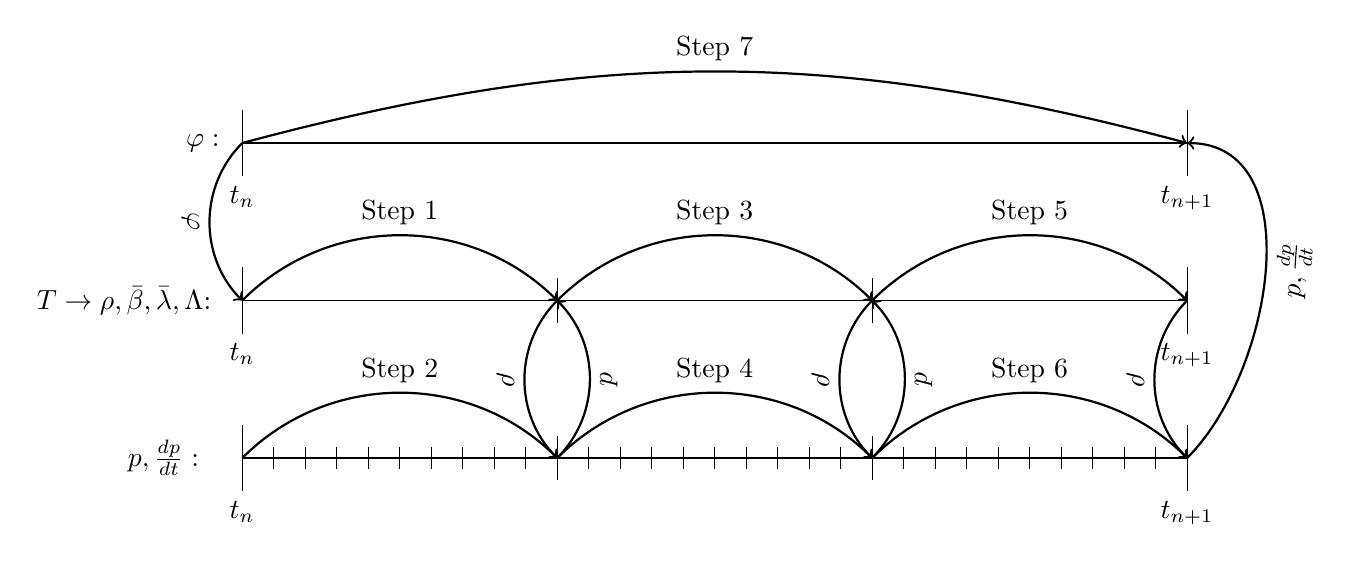
\begin{tikzpicture}[scale=2]
%Shape
\draw[] (0,2) -- (6,2) ;
\foreach \x in  {0,6}
\draw[shift={(\x,2)},color=black] (0pt,6pt) -- (0pt,-6pt);
\draw[shift={(0,2)},color=black] (0pt,0pt) -- (0pt,-6pt) node[below] {$t_n$};
\draw[shift={(6,2)},color=black] (0pt,0pt) -- (0pt,-6pt) node[below] {$t_{n+1}$};
\node(shape) at (-.25,2) {$\varphi:$};

%Temp/Params
\draw[] (0,1) -- (6,1) ;
\foreach \x in  {0,6}
\draw[shift={(\x,1)},color=black] (0pt,6pt) -- (0pt,-6pt);
\foreach \x in  {2,4}
\draw[shift={(\x,1)},color=black] (0pt,4pt) -- (0pt,-4pt);
\draw[shift={(0,1)},color=black] (0pt,0pt) -- (0pt,-6pt) node[below] {$t_n$};
\draw[shift={(6,1)},color=black] (0pt,0pt) -- (0pt,-6pt) node[below] {$t_{n+1}$};
\node(temp) at (-.75,1) {$T \rightarrow \rho, \bar{\beta}, \bar{\lambda}, \Lambda$:};

% PRKE
\draw[] (0,0) -- (6,0) ;
\foreach \x in  {0,6}
\draw[shift={(\x,0)},color=black] (0pt,6pt) -- (0pt,-6pt);
\foreach \x in  {0,2,4,6}
\draw[shift={(\x,0)},color=black] (0pt,4pt) -- (0pt,-4pt);
\foreach \x in  {0,0.2,0.4,0.6,0.8,1,1.2,1.4,1.6,1.8,2,2.2,2.4,2.6,2.8,3,3.2,3.4,3.6,3.8,4,4.2,4.4,4.6,4.8,5,5.2,5.4,5.6,5.8,6}
\draw[shift={(\x,0)},color=black] (0pt,2pt) -- (0pt,-2pt);
\draw[shift={(0,0)},color=black] (0pt,0pt) -- (0pt,-6pt) node[below] {$t_n$};
\draw[shift={(6,0)},color=black] (0pt,0pt) -- (0pt,-6pt) node[below] {$t_{n+1}$};
\node(prke) at (-.5,0) {$p, \frac{dp}{dt}:$};

\draw (0,0) edge[out=45,in=135,->,thick] node[above,sloped] {Step 2} (2,0);
\draw (2,0) edge[out=45,in=135,->,thick] node[above,sloped] {Step 4} (4,0);
\draw (4,0) edge[out=45,in=135,->,thick] node[above,sloped] {Step 6} (6,0);
\draw (0,1) edge[out=45,in=135,->,thick] node[above,sloped] {Step 1} (2,1);
\draw (2,1) edge[out=45,in=135,->,thick] node[above,sloped] {Step 3} (4,1);
\draw (4,1) edge[out=45,in=135,->,thick] node[above,sloped] {Step 5} (6,1);
\draw (0,2) edge[out=15,in=165,->,thick] node[above,sloped] {Step 7} (6,2);

\draw (0,2) edge[out=-135,in=135,->,thick] node[below,sloped] {$\varphi$} (0,1);
\draw (2,1) edge[out=-135,in=135,->,thick] node[below,sloped] {$\rho$} (2,0);
\draw (2,0) edge[out=45,in=-45,->,thick] node[below,sloped] {$p$} (2,1);
\draw (4,1) edge[out=-135,in=135,->,thick] node[below,sloped] {$\rho$} (4,0);
\draw (4,0) edge[out=45,in=-45,->,thick] node[below,sloped] {$p$} (4,1);
\draw (6,1) edge[out=-135,in=135,->,thick] node[below,sloped] {$\rho$} (6,0);
\draw (6,0) edge[out=45,in=0,->,thick] node[below,sloped] {$p, \frac{dp}{dt}$} (6,2);

\end{tikzpicture}
}
\caption{Time scales and process of IQS with temperature feedback}
\label{fig:time}
\end{figure}

Iteration processes are needed for each time scale.  The amplitude and temperature need to be iterated on the middle time scale until convergence on each temperature step.  Then another iterative process needs to occur in the shape time scale on all three variables. \fig{fig:proc} shows the programming diagram implement to execute this process. The time increment of $\Delta t/3$ for the temperature solve is arbitrary and is meant only to match \fig{fig:time} where three temperature updates have been used as illustration.

\begin{figure}[!htpb]
\centering
\resizebox{\linewidth}{!}{
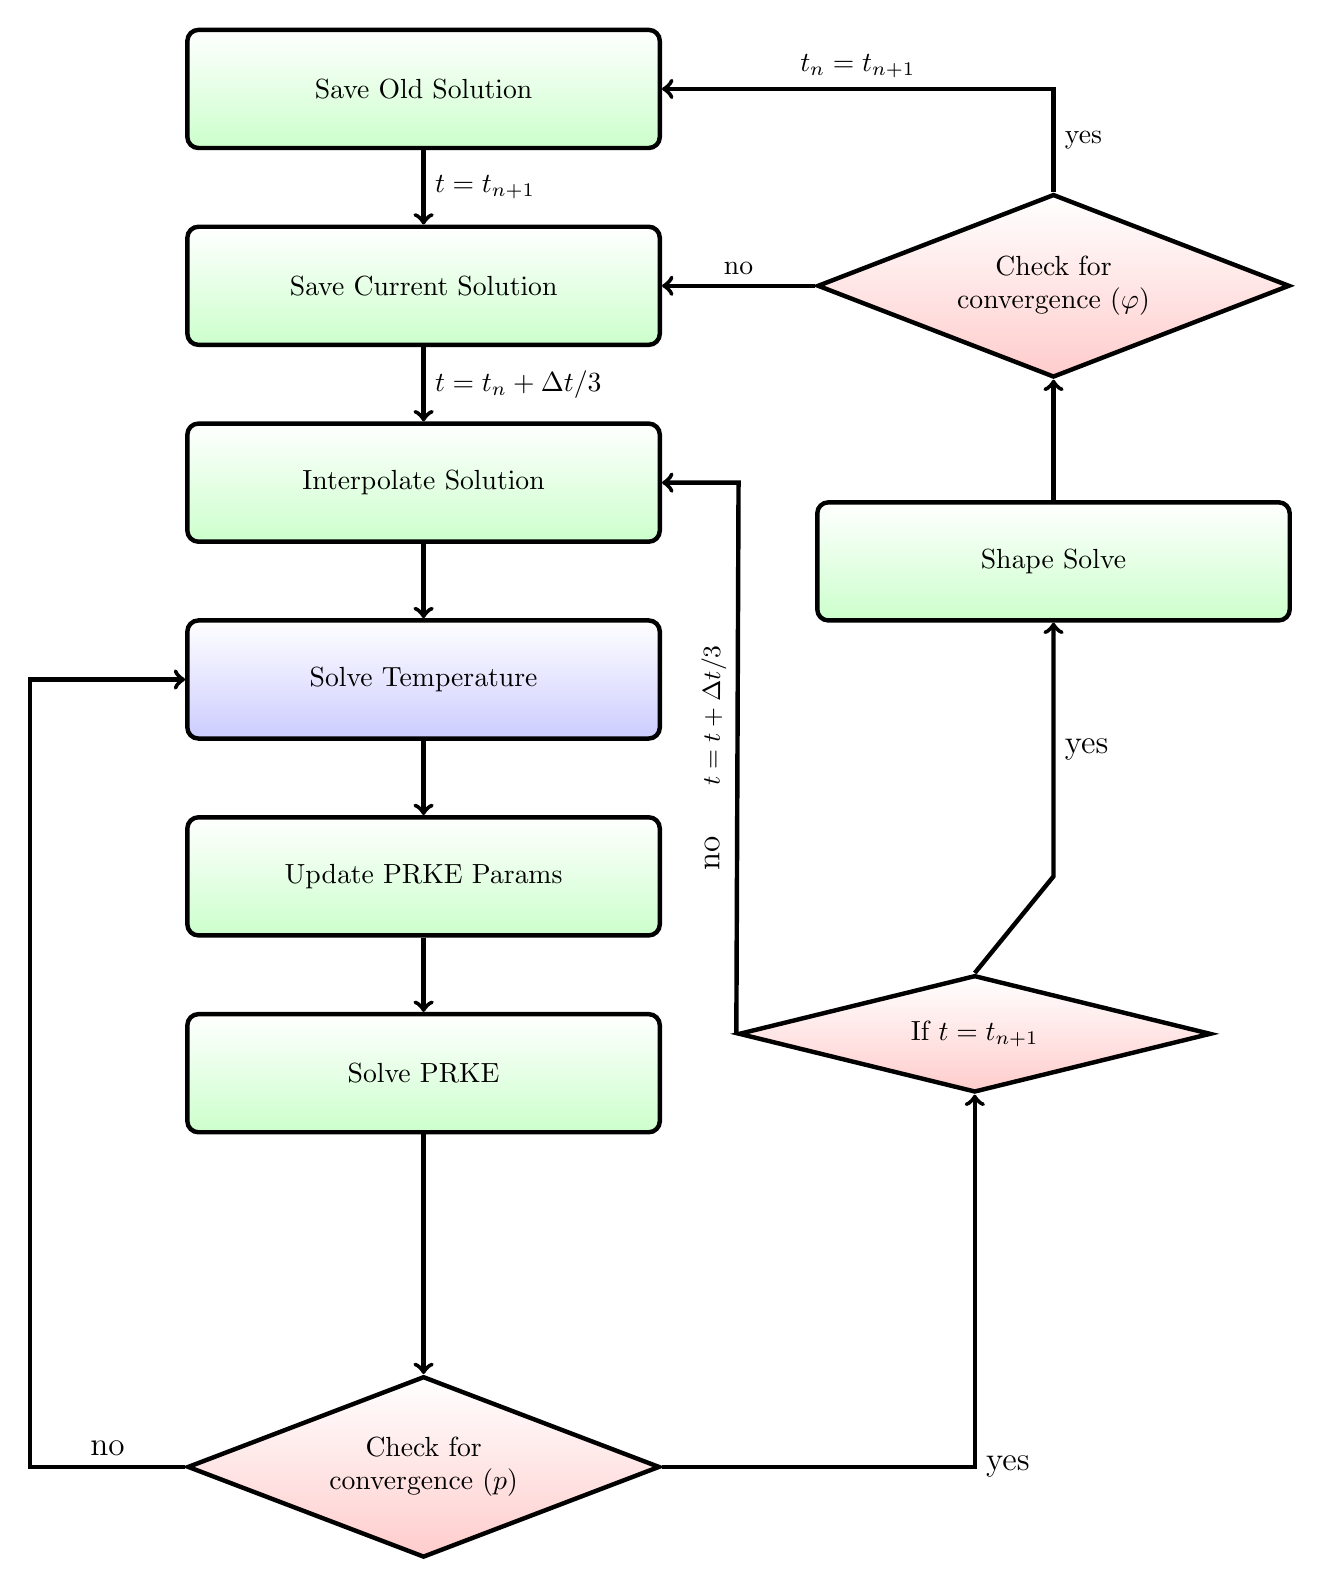
\begin{tikzpicture}[every node/.style = {font=\normalsize}]

\node[greenblock](p1) at (0,0) {Save Old Solution};
\node[greenblock](p2) at (0,-2.5) {Save Current Solution};
\node[greenblock](p3) at (0,-5) {Interpolate Solution};
\node[blueblock2](p4) at (0,-7.5) {Solve Temperature};
\node[greenblock] (p5) at (0,-10) {Update PRKE Params};
\node[greenblock] (p6) at (0,-12.5) {Solve PRKE};
\node[reddiamond] (check1) at (0,-17.5) {Check for \\ convergence ($p$)};
\node[reddiamond] (check2) at (7,-12) {If $t=t_{n+1}$};
\node[greenblock] (p7) at (8,-6) {Shape Solve};
\node[reddiamond] (check3) at (8,-2.5) {Check for \\ convergence ($\varphi$)};
%\node [above =0.1mm of p1] {\large{IQS Solve:}};
%\node [above =0.1mm of p5] {\large{Multi-physics:}};

%\tikzback{p1}{p1}{p4}{p4}{bk1}
%\tikzback{p5}{p5}{p5}{p5}{bk2}

\draw[->,ultra thick](p1.south) -- node[right] {$t=t_{n+1}$}(p2.north);
\draw[->,ultra thick](p2.south) -- node[right] {$t=t_{n}+\Delta t/3$}(p3.north);
\draw[->,ultra thick](p3.south) -- (p4.north);
\draw [->,ultra thick] (p4.south)-- (p5.north);
\draw[->,ultra thick](p5.south) -- (p6.north);
\draw[->,ultra thick](p6.south) -- (check1.north);
\draw[->,ultra thick](check1.west) -- node[above,sloped] {\large{no}} (-5,-17.5) |-  (p4.west);
\draw[->,ultra thick](check1.east) -| node[right] {\large{yes}} (check2.south);
\draw[->,ultra thick](check2.west) -- node[above,sloped] {\large{no}\small \qq $t=t+\Delta t/3$} (4,-5) -- (p3.east);
\draw[->,ultra thick](check2.north) --  (8,-10) -- node[right] {\large{yes}} (p7.south);
\draw[->,ultra thick](p7.north) -- (check3.south);
\draw[->,ultra thick](check3.west) -- node[above] {no} (p2.east);
\draw[->,ultra thick](check3.north) -- node[right] {yes} (8,0) -- node[above] {$t_n=t_{n+1}$} (p1.east);

\end{tikzpicture}
}
\caption{Visualization of fixed-point iteration and temperature update process for IQS}
\label{fig:proc}
\end{figure}

%---------------------------------------------------------------------------------------%
\subsection{Delayed Neutron Precursor Treatment}
%---------------------------------------------------------------------------------------%

This section presents the time-integration method used to solve coupled flux/shape and precursor equations, represented by Equations~\eqref{eq:flux}/\eqref{eq:shape}~and~\eqref{eq:precursor}/\eqref{eq:prec}. First, we note that we could keep this system of two time-dependent equations and solve it as a coupled system. However, this is unnecessary and a memory expensive endeavor because the precursor equation is only an ODE and not a PDE. Instead, one may discretize in time the shape equation, which typically requires the knowledge of the precursor concentrations at the end of the time step. This precursor value is taken from the solution, numerical or analytical, of the precursors ODE.

A common precursor evaluation technique is using the theta method; applying this to \eqt{eq:prec}:

\be
C^{n+1} = \frac{1-(1-\theta)\Delta t\lambda}{1+\theta\Delta t\lambda}C^n + \frac{(1-\theta)\Delta t \beta}{1+\theta\Delta t\lambda}S_f^n p^n +  \frac{\theta\Delta t \beta}{1+\theta\Delta t\lambda}S_f^{n+1} p^{n+1}
\label{eq:dnp_theta}
\ee

Where $S_f$ is the fission source equivalent for shape ($S_f^n=(\nu\Sigma_f)^n\varphi^n$). Another technique to evaluating the precursor equation is to use a exponential operator and integrate the time derivative analytically.  Applying this operation to \eqt{eq:prec} yields:

\be
C^{n+1} =  C^n e^{-\lambda (t_{n+1} - t_n) }  + \int_{t_n}^{t_{n+1}} \beta(t') S_f(t') p(t')e^{-\lambda (t_{n+1}-t')}dt'
\label{eq:prec_an}
\ee

Again, this can be applied to implicit discretization by altering the definition of the fission source and eliminating $p$.  Because $S_f$ is not known continuously over the time step, the integration can be done using any scheme (Riemann, trapezoid, Simpson's, etc.). However, there is a very accurate representation of $p(t)$ over the macro step from the PRKE solve. In order to utilize this information, another possibility is to interpolate $S_f$ linearly over the macro step.  Such that:

\be
S_f(t) = \frac{t_{n+1}-t}{t_{n+1}-t_n}S_f^n  + \frac{t-t_n}{t_{n+1}-t_n}S_f^{n+1}  \quad t_n \le t \le t_{n+1}
\ee
Applying this to \eqt{eq:prec_an} yields:
\be
C^{n+1} = C^n e^{-\lambda \Delta t} + \left(\hat{a}_2 S_f^{n+1}+\hat{a}_1 S_f^n\right)\beta
\label{eq:dnp_an}
\ee

With integration coefficients defined as:

\begin{align}
&\hat{a}_1= \int_{t_n}^{t_{n+1}}\frac{t_{n+1}-t'}{\Delta t}p(t')e^{-\lambda(t_{n+1}-t')}dt' \\
&\hat{a}_2 = \int_{t_n}^{t_{n+1}}\frac{t'-t_n}{\Delta t}p(t')e^{-\lambda(t_{n+1}-t')}dt'
\end{align}


%---------------------------------------------------------------------------------------%
\subsection{Step Doubling Time Adaptation}
%---------------------------------------------------------------------------------------%

Further enhancements to IQS performance can be gained by using time adaptation (or time step control) in order to increase or reduce the macro time step size for the shape evaluation, depending on error estimates. A step-doubling technique is chosen as the time adaptation technique \cite{NumC}. The step doubling technique involves estimating the local error for a certain time step by taking the difference between a solution with one full step ($\varphi^g_{\Delta t}$) and a solution with two half steps ($\varphi^g_{\Delta t/2}$). Note: $\varphi$ is changed to $\phi$ for implicit discretization and IQS P-C.

The relative error is computed as follows:
\be
e_n = \frac{\norm{\sum_{g=1}^G\varphi^g_{\Delta t/2} - \sum_{g=1}^G\varphi^g_{\Delta t}}}{\text{max}\left(\norm{\sum_{g=1}^G\varphi^g_{\Delta t/2}},\norm{\sum_{g=1}^G\varphi^g_{\Delta t}}\right)}
\label{eq:edt2}
\ee
If the error is smaller than the user-specified tolerance, $e_{tol}$, the time step is accepted. In addition, a new time step size is estimated as follows:
\be
\Delta t_{new} = S \Delta t \left(\frac{e_{tol}}{e_n}\right)^{\frac{1}{1+q}}
\label{eq:dt2}
\ee

Where $q$ is the convergence order of the time integration scheme being used and $S\simeq 0.8$ is a safety factor. If the error is larger than the user-specified tolerance, the time step is rejected. A new time step size is estimated using  \eqt{eq:edt2} as well. This process can be visualized by \figs{fig:dt2_1}{fig:dt2_2}.  Where a step involves a full convergence of shape, amplitude, and any multiphysics on the respective time step.

To investigate IQS's performance with step-doubling time adaptation, the adaptation will be applied to implicit discretization method, traditional IQS, and IQS P-C.  Each of these methods will be applied to several diffusion problems; the number of time steps taken and the resulting error will be used to compare the methods.

\begin{figure}[htpb!]
\centering
\resizebox{\linewidth}{!}{
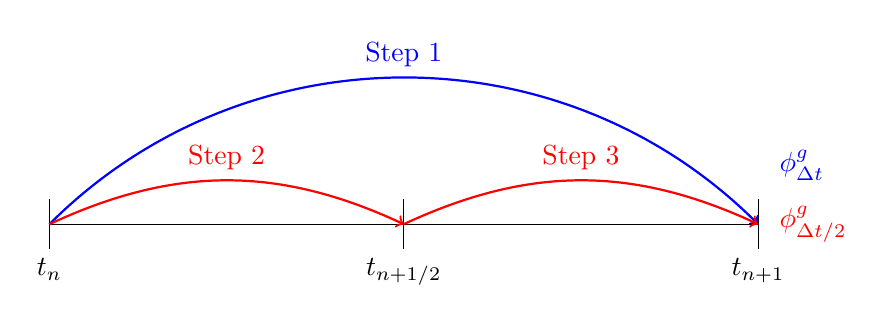
\begin{tikzpicture}[scale=1.5]
\draw[] (0,2) -- (6,2) ;
\foreach \x in  {0,3,6}
\draw[shift={(\x,2)},color=black] (0pt,6pt) -- (0pt,-6pt);
\draw[shift={(0,2)},color=black] (0pt,0pt) -- (0pt,-6pt) node[below] {$t_n$};
\draw[shift={(3,2)},color=black] (0pt,0pt) -- (0pt,-6pt) node[below] {$t_{n+1/2}$};
\draw[shift={(6,2)},color=black] (0pt,0pt) -- (0pt,-6pt) node[below] {$t_{n+1}$};
\draw (0,2) edge[out=45,in=135,->,thick,blue] node[above,sloped] {\tcb{Step 1}} (6,2);
\draw (0,2) edge[out=25,in=155,->,thick,red] node[above,sloped] {\tcr{Step 2}} (3,2);
\draw (3,2) edge[out=25,in=155,->,thick,red] node[above,sloped] {\tcr{Step 3}} (6,2);
\node[anchor=west](shape) at (6.1,2.5) {$\tcb{\phi_{\Delta t}^g}$};
\node[anchor=west](shape) at (6.1,2) {$\tcr{\phi_{\Delta t/2}^g}$};

\end{tikzpicture}
}
\caption{Visualization of step doubling process on time-line}
\label{fig:dt2_1}
\end{figure}

\begin{figure}[!htpb]
\centering
\resizebox{\linewidth}{!}{
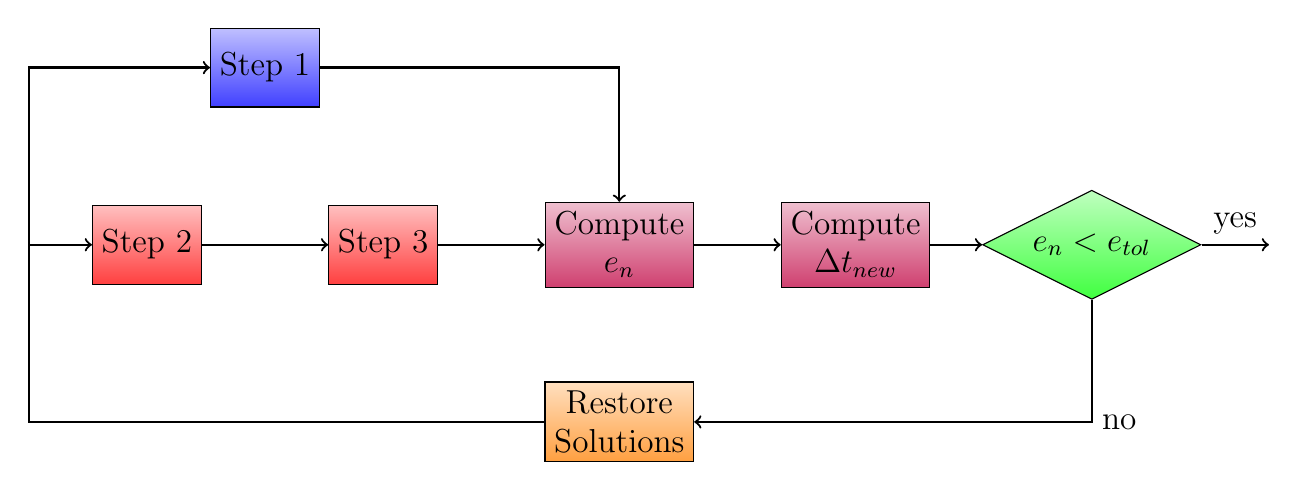
\begin{tikzpicture}[every node/.style = {font=\large},scale=0.75]

\node[blueblock](p1) at (-6,3) {Step 1} ;
\node[redblock](p2) at (-8,0) {Step 2} ;
\node[redblock](p3) at (-4,0) {Step 3} ;
\node[purpleblock](p4) at (0,0) {Compute \\ $e_n$};
\node[purpleblock](p5) at (4,0) {Compute  \\ $\Delta t_{new}$};
\node[greendiamond](p6) at (8,0) {$e_n < e_{tol}$};
\node[orangeblock](p7) at (0,-3) {Restore \\ Solutions};

\draw[->,thick](p1.east) -| (p4.north);
\draw[->,thick](p2.east) -- (p3.west);
\draw[->,thick](p3.east) -- (p4.west);
\draw[->,thick](p4.east) -- (p5.west);
\draw[->,thick](p5.east) -- (p6.west);
\draw[->,thick](p6.south) |- node[right] {no} (p7.east);
\draw[->,thick](p6.east) -- node[above] {yes} (11,0);
\draw[->,thick](p7.west) -| (-10,0) -- (p2.west);
\draw[->,thick](p7.west) -| (-10,0) |- (p1.west);

\end{tikzpicture}
}
\caption{Visualization of step doubling process with coding logic}
\label{fig:dt2_2}
\end{figure}


%%%%%%%%%%%%%%%%%%%%%%%%%%%%%%%%%%%%%%%%%%%%%%%%%%%%%%%%%%%%%%%%%%%%%%%%%%%%%%%%%%%%%%%%%
\section{Kinetics Results}
%%%%%%%%%%%%%%%%%%%%%%%%%%%%%%%%%%%%%%%%%%%%%%%%%%%%%%%%%%%%%%%%%%%%%%%%%%%%%%%%%%%%%%%%%

This section describes kinetics examples that IQS is tested with and analysis of its performance.  The examples range in complexity and application.  The first is a one-dimensional problem, designed for the prototype code in MATLAB.  The next one is from the Argonne National Lab (ANL) Benchmark Problem Book (BPB), and is a common problem for testing codes and developing methods \cite{ANL_BPB}.

%---------------------------------------------------------------------------------------%
\subsection{One-Dimensional Problem}
%---------------------------------------------------------------------------------------%

This example is very simple and computes quickly; it entails a one dimensional, homogeneous 400 cm slab with a heterogenous perturbation in absorption cross section.  \fig{fig:slab} shows how the regions of the slab are divided and \tbl{tab:1Dmat} shows the initial material properties.  Regions 2, 3, and 4 have slope perturbations at different points in time, \tbl{tab:1Dslope} shows the values of the absorption cross-section in each region at the times of interest.  The values of $\Sigma_a$ between these times of interest are linear interpolations between the given values.

\begin{figure}[!htbp]
\begin{center}
\resizebox{\linewidth}{!}{
\begin{tabular}{| l | l | l | l | l | l | l | l | l | l | l | l | l | l | l | l | l | l | l | l |}
\hline \hline \hline
  &   &   &   &   &   &    &    &   &   &   &   &   &   &   &   &   &   &   &   \\
1 & 1 & 1 & 1 & 2 & 3 & 1 & 1 & 1 & 1 & 1 & 1 & 1 & 1 & 4 & 4 & 1 & 1 & 1 & 1 \\
  &   &   &   &   &   &    &    &   &   &   &   &   &   &   &   &   &   &   &   \\
\hline \hline \hline
\end{tabular}
}
\caption{1-D slab region identification}
\label{fig:slab}
\end{center}
\end{figure}

\begin{table}[!htbp]
\begin{center}
\caption{1-D slab material properties and problem parameters}
\label{tab:1Dmat}
\resizebox{\linewidth}{!}{
\begin{tabular}{llllll}
\hline
$D (cm)$ & $\Sigma_a (cm^{-1})$ & $\nu \Sigma_f (cm^{-1})$ & $v (cm/s)$ & $\beta$ & $\lambda (s^{-1})$ \\
\hline
1.0 & 1.1 & 1.1 & 1,000 & 0.006 & 0.1 \\

\hline
\end{tabular}
}
\end{center}
\end{table}

\begin{table}[!htbp]
\begin{center}
\caption{1-D slab absorption cross-section at times of interest}
\label{tab:1Dslope}
\resizebox{\linewidth}{!}{
\begin{tabular}{llllllll}
\hline
Region & Material Property & 0.0 s & 0.1 s & 0.6 s & 1.0 s & 1.7 s \\
\hline
2 & $\Sigma_{a} (cm^{-1})$ & 1.1 & 1.1 & 1.095 & 1.095 & 1.095 \\
3 & $\Sigma_{a} (cm^{-1})$ & 1.1 & 1.1 & 1.09 & 1.09 & 1.1 \\
4 & $\Sigma_{a} (cm^{-1})$ & 1.1 & 1.1 & 1.105 & 1.105 & 1.105 \\
\hline
\end{tabular}
}
\end{center}
\end{table}

\fig{fig:1D_flux} shows the resulting baseline flux and relative power profile of the one-dimensional problem.  The baseline was computed using MATLAB's ode15s function which is a embedded Runge-Kutta time adaptive method for stiff problems, the error tolerance was set very tightly ($10^{-12}$).  The flux distribution shows that the core is relatively large, thus different regions are weakly coupled. This baseline computation is used to compute the error of the other time discretization methods.  \fig{fig:1D_shape} shows the shape profile at various times during the transient.  It is apparent that the shape is very time-dependent, so it is expected that IQS has marginal accuracy gain for a given time step size.

\begin{figure}[!htbp]
\centering
\begin{subfigure}[b]{\linewidth}
\centering
\includegraphics[width=\linewidth]{figures/1D_flux.png}
\caption{Flux profile at various times}
\end{subfigure}
\begin{subfigure}[b]{\linewidth}
\centering
\includegraphics[width=\linewidth]{figures/1D_power_base.png}
\caption{Power profile over transient}
\end{subfigure}
\caption{Baseline flux and power distribution}
\label{fig:1D_flux}
\end{figure}

\begin{figure}[!htbp]
\centering
\begin{subfigure}[b]{\linewidth}
\centering
\includegraphics[width=\linewidth]{figures/1D_shape2.png}
\caption{Shape profile at various times}
\label{fig:1D_shape}
\end{subfigure}
\begin{subfigure}[b]{\linewidth}
\centering
\includegraphics[width=\linewidth]{figures/1D_iqs_power.png}
\caption{Power and reactivity profile over transient}
\end{subfigure}
\caption{IQS flux and power distribution}
\label{fig:1D_res}
\end{figure}


%----------------------------------------------------------------------------------------
\subsubsection{Iteration Analysis}

IQS, as previously stated, is a system of nonlinear equations between shape and amplitude. These equations needed to be iterated to numerically converge to an accurate solution.  \sct{sect:iter} lists various iteration techniques for fixed-point and Newton schemes. \fig{fig:iter} shows the number of fixed-point iterations required for a $10^{-11}$ tolerance over the transient. The criteria listed in the legend correspond to the list as such:
\begin{enumerate}
\item $L^{\infty} \rightarrow$ 1.
\item $L^{2} \rightarrow$ 2.
\item Reactivity $\rightarrow$ 3.
\item Amplitude $\rightarrow$ 4.
\item K criteria $\rightarrow$ 5.
\item All properties $\rightarrow$ 3.-5.
\end{enumerate}
This plot shows that 1-4 have approximately the same convergence behavior, but the K criteria converges to a certain error. \fig{fig:iter_err} shows the resulting error the K criteria converges to for different points of rescaling the shape. The rescaling is described by \eqt{eq:shape_scale}. Rescaling shape more frequently helps the error.  However, rescaling every iteration is somewhat artificial because it does not consider changes spatially. Regardless, an error of $~10^{-5}$ is quite large and it is expected that the magnitude is due to the explicit treatment of precursors (\eqt{eq:dnp_theta}). Switching to an analytical elimination (\eqt{eq:dnp_an}) does not converge as well, but the error is much smaller, seen in \fig{fig:iter_err_an}.

\begin{figure}[!htbp]
\centering
\includegraphics[width=\linewidth]{figures/iter_renorm.png}
\caption{\# of iterations for various convergence criteria, tolerance$=10^{-11}$, max iterations$=20$}
\label{fig:iter}
\end{figure}

\begin{figure}[!htbp]
\centering
\includegraphics[width=\linewidth]{figures/iter_error.png}
\caption{Final iteration error for K convergence criteria}
\label{fig:iter_err}
\end{figure}

\begin{figure}[!htbp]
\centering
\includegraphics[width=\linewidth]{figures/iter_error_an.png}
\caption{Final iteration error for K convergence criteria with analytical precursor elimination}
\label{fig:iter_err_an}
\end{figure}

%----------------------------------------------------------------------------------------
\subsubsection{One-Dimensional Problem Time Step Convergence Analysis}

Time step convergence analysis involves evaluating a problem with various refinements in step size and comparing the resulting errors with the time step size. Plotting error versus $\Delta t$ on a log-scale should produce a relatively strait line with a slope equal to the order of the time discretization method. In order to evaluate the performance and error convergence of IQS, the slab was simulated with varying time discretization methods and time step sizes.  \fig{fig:1D_conv} shows these convergence plots of five different discretization methods for implicit discretization, IQS, and IQS P-C.  These plots were generated from the results using the MATLAB prototype program.  The plots show that IQS and IQS P-C are convergent through fourth order BDF.  Third order SDIRK did not show third order convergence, but, through extensive testing, SDIRK shows non-convergent behavior for too stiff of problems.  

There are higher discretization order that can be tested, but most practical application do not go beyond second order.  This paper shows an analysis of the first publicized application of IQS with higher than second order discretization, which exposed unforeseen properties of IQS.  When using higher order techniques, the interpolation of PRKE parameters and shape for precursor integration become important to consider.  Every other application that was investigated linearly interpolates parameters for the PRKE evaluation.  Similarly, the shape used for the integration of the ODE for the precursors needs to have higher order interpolation to preserve high order error convergence.  This interpolation was done using Lagragian and Hermite methods, both leading to successful convergence.

\begin{figure*}[!htbp]
\centering
\begin{subfigure}[b]{0.49\textwidth}
\centering
\includegraphics[width=\linewidth]{figures/1D_conv_IE.png}
\caption{Implicit Euler}
\end{subfigure}
\begin{subfigure}[b]{0.49\textwidth}
\centering
\includegraphics[width=\linewidth]{figures/1D_conv_BDF2.png}
\caption{BDF2}
\end{subfigure}
\begin{subfigure}[b]{0.49\textwidth}
\centering
\includegraphics[width=\linewidth]{figures/1D_conv_BDF3.png}
\caption{BDF3}
\end{subfigure}
\begin{subfigure}[b]{0.49\textwidth}
\centering
\includegraphics[width=\linewidth]{figures/1D_conv_BDF4.png}
\caption{BDF4}
\end{subfigure}
\begin{subfigure}[b]{0.49\textwidth}
\centering
\includegraphics[width=\linewidth]{figures/1D_conv_SDIRK33.png}
\caption{SDIRK33}
\end{subfigure}
\caption{Error convergence plots of implicit discretization, IQS, and IQS P-C with various time discretization schemes}
\label{fig:1D_conv}
\end{figure*}

%----------------------------------------------------------------------------------------
\subsubsection{One-Dimensional Mini-Core Problem}

This problem is exactly the same as the previous one-dimensional problem, except the the core was reduced to 80 cm in length. The purpose of testing this problem is to determine if a more tightly coupled core will yield better performance for IQS. \fig{fig:1Dmini_flux} shows the resulting baseline flux and relative power profile of the one-dimensional mini-core problem. This plot shows that the perturbed regions affect the domain more evidently. \fig{fig:1Dmini_shape} shows the shape profile at various times during the transient. This plot shows that the shape is much less time-dependent than the previous large core. \fig{fig:1Dmini_conv} shows that IQS performs significantly better with this example than the large core.

\begin{figure}[!htbp]
\centering
\begin{subfigure}[b]{\linewidth}
\centering
\includegraphics[width=\linewidth]{figures/1Dmini_flux.png}
\caption{Flux profile at various times}
\end{subfigure}
\begin{subfigure}[b]{\linewidth}
\centering
\includegraphics[width=\linewidth]{figures/1Dmini_power_base.png}
\caption{Power profile over transient}
\end{subfigure}
\caption{Mini-core baseline flux and power distribution}
\label{fig:1Dmini_flux}
\end{figure}

\begin{figure}[!htbp]
\centering
\includegraphics[width=\linewidth]{figures/1Dmini_shape.png}
\caption{Shape profile at various times for one-dimensional mini-core}
\label{fig:1Dmini_shape}
\end{figure}

\begin{figure}[!htbp]
\centering
\includegraphics[width=\linewidth]{figures/1Dmini_conv_IE.png}
\caption{Time step convergence for one-dimensional mini-core with implicit Euler discretization}
\label{fig:1Dmini_conv}
\end{figure}

%---------------------------------------------------------------------------------------%
\subsection{TWIGL Benchmark}
%---------------------------------------------------------------------------------------%

This benchmark problem originates from the Argonne National Lab Benchmark Problem Book \cite{ANL_BPB}.  It is a 2D, 2-group reactor core model with no reflector region \cite{TWIGL_benchmark}.  This example is meant to be of progressive complexity from the previous example.  The transient of this reactor is very geometrically symmetrical with very little temporal shape change.  Therefore, IQS is expected to perform significantly better than the implicit discretization method. Figs. \ref{fig:TWIGL_power} show the IQS  solution as compared with the implicit discretization solution. This shows that IQS is consistent in more complex, higher dimensional problems. These plots also serve to illustrate that IQS has a much more accurate solution, even at a significantly larger time step than the implicit discretization.

\begin{figure}[!htbp]
\centering
\begin{subfigure}[!htbp]{0.49\textwidth}
\includegraphics[width=\textwidth]{figures/TWIGL_power_plot.png}
\caption{Power profile for entire transient}
\end{subfigure}
\begin{subfigure}[!htbp]{0.49\textwidth}
\includegraphics[width=\textwidth]{figures/TWIGL_power_plot2.png}
\caption{Power at cusp of profile}
\end{subfigure}
\caption{Power level comparison of TWIGL Benchmark}
\label{fig:TWIGL_power}
\end{figure}

%----------------------------------------------------------------------------------------
\subsubsection{TWIGL Time Step Convergence Analysis}

In order to demonstrate asymptotic convergence of IQS, implicit Euler (IE) and second order BDF (BDF2) were applied to the TWIGL simulation. \fig{fig:TWIGL_conv} plots the error convergence of IQS and the implicit discretization methods.  The curves show the impressive convergence of IQS for the highly transient TWIGL example. The slope indicated in the legend are the linear slope of curves on the log plot, these slopes should be similar to the order of the method (1 for IE and 2 for BDF2).  IQS shows a increased order because the PRKE is performing much of accuracy convergence and it is computed using SDIRK33, a third order method.

\begin{figure}[!htbp]
\centering
\includegraphics[width=\linewidth]{figures/TWIGL_convergence.jpg}
\caption{Error convergence comparison of TWIGL Benchmark}
\label{fig:TWIGL_conv}
\end{figure}

%----------------------------------------------------------------------------------------
\subsubsection{TWIGL Time Adaptation}

\tbl{tab:TWIGLdt2} and \fig{fig:TWIGL_power_dt2} show the results for TWIGL with time adaptation.  The results show that both IQS methods perform exceptionally well compared to implicit discretization.  It also shows that traditional IQS performed better with large $e_{tol}$, while IQS P-C was better with smaller $e_{tol}$.

\begin{table*}[!htbp]
\begin{center}
\caption{TWIGL step doubling results}
\label{tab:TWIGLdt2}
%\resizebox{\linewidth}{!}{
\begin{tabular}{|l|l|l|l|l|l|l|l|l|l|l|}
\hline
  &  & \multicolumn{3}{|c|}{Implicit Discretization} & \multicolumn{3}{|c|}{IQS} & \multicolumn{3}{|c|}{IQS P-C} \\
\hline
Test & $e_{tol}$ & Error & Steps & Solves & Error & Steps & Solves & Error & Steps & Solves \\
\hline
1 &	0.05    &	0.00012677 &	9   &	29  &	0.03380433 &	4   &	20   &	0.00323100 &	4  &	9   \\
2 &	0.01    &	3.5555e-05 &	11  &	35  &	0.00166991 &	5   &	40   &	0.00263068 &	5  &	12  \\
3 &	0.005   &	4.0364e-05 &	11  &	31  &	0.00886584 &	5   &	40   &	0.00160486 &	6  &	21  \\
4 &	0.001   &	0.00294822 &	33  &	122 &	0.02976305 &	5   &	36   &	1.7527e-05 &	10 &	35  \\
5 &	0.0005  &	0.00099778 &	39  &	131 &	0.00143781 &	6   &	55   &	1.4185e-05 &	16 &	74  \\
6 &	0.0001  &	0.00019510 &	78  &	236 &	0.00016175 &	8   &	65   &	6.2903e-06 &	19 &	78  \\
7 &	5.0e-05 &	0.00018372 &	112 &	342 &	6.0328e-05 &	12  &	163  &	1.5247e-06 &	24 &	92  \\
8 &	1.0e-05 &	8.0564e-05 &	263 &	794 &	7.7103e-05 &	379 &	5729 &	9.8321e-07 &	48 &	210 \\
\hline

\end{tabular}%}
\end{center}
\end{table*}

\begin{figure}[!htbp]
\centering
\includegraphics[width=\linewidth]{figures/TWIGL_power_plot_dt2.png}
\caption{Power level comparison of TWIGL Benchmark with time adaptation}
\label{fig:TWIGL_power_dt2}
\end{figure}

%---------------------------------------------------------------------------------------%
\subsection{LMW Benchmark?}
%---------------------------------------------------------------------------------------%

%%%%%%%%%%%%%%%%%%%%%%%%%%%%%%%%%%%%%%%%%%%%%%%%%%%%%%%%%%%%%%%%%%%%%%%%%%%%%%%%%%%%%%%%%
\section{Dynamics Results}
%%%%%%%%%%%%%%%%%%%%%%%%%%%%%%%%%%%%%%%%%%%%%%%%%%%%%%%%%%%%%%%%%%%%%%%%%%%%%%%%%%%%%%%%%

This section describes two dynamics examples, including the LRA benchmark and a TREAT experiment.  These examples are of increased complexity from the previous kinetics examples.  This section also analyzes IQS's performance with these, which is vital for verification of IQS in real-world problems.

%---------------------------------------------------------------------------------------%
\subsection{LRA Benchmark}
%---------------------------------------------------------------------------------------%

The LRA benchmark is a two-dimensional, two-group neutron diffusion problem with adiabatic heat-up and Doppler feedback in thermal reactor.  It is a super prompt-critical transient. The execution of the benchmark was performed by the Rattlesnake/MOOSE framework at Idaho National Laboratory (INL) \cite{wang2013}.  The spacial discretization was performed using continuous finite element method with first order Lagrangian basis functions. The mesh consisted of blocks $11\times 11$ with five uniform refinements, totaling $165,165$ elements and $124,609$ nodes. Three different temporal techniques were applied: implicit discretization of the flux equation, IQS, and IQS-PC. Crank-Nicholson time discretization scheme was used for the diffusion evaluation of each technique.  Third order Runge-Kutta discretization with step doubling adaptation was used for the PRKE evaluation.  The performance of IQS and the temperature updates were measured by its improvement in accuracy at peak power over the implicit discretization method.

\fig{fig:lra_profile} shows the baseline power and temperature transient profile for the LRA benchmark. The baseline results are compared to the results achieved by Sutton and Aviles in \cite{Sutton_1996} and presented in \tbl{tab:base}.  The relative difference in the magnitude of the peak power ($t\approx1.44 s$) from the baseline was used for error comparison.  

\begin{figure}[htbp!]
\centering
\includegraphics[width=\linewidth]{figures/lra_profile.png}
\caption{LRA baseline temperature and power profile}
\label{fig:lra_profile}
\end{figure}

\begin{table}[!htbp]
\begin{center}
\caption{LRA baseline verification}
\label{tab:base}
\resizebox{\linewidth}{!}{
\begin{tabular}{|l|cc|}
\hline
Calculation  &  Baseline & Sutton (Spandex 1936) \\
\hline
No. of Spatial Nodes	& 3872 		& 1936 \\
Eigenvalue 				& 0.99637	& 0.99637 \\
No. of Time Steps 		& 6000 		& 23,890 \\
Time to Peak Power (s) 	& 1.441 	& 1.441 \\
Peak Power (W/cm$^3$) 	& 5456 		& 5461 \\
\hline
\end{tabular}
}
\end{center}
\end{table}

%----------------------------------------------------------------------------------------
\subsubsection{LRA Results}

This section shows the time step error convergence of IQS for the LRA benchmark, as well as the effect of the intermediate temperature time scale. \fig{fig:lra_bad} is an error convergence plot comparing the three techniques where temperature is evaluated only on the macro step (1 temperature update).  \fig{fig:lra_mpconv} is an error convergence plot comparing the three techniques where temperature is evaluated 5 times within a macro step (5 temperature updates).  Finally, \fig{fig:mp} shows the effect of various temperature updates. The dashed lines correspond to implicit discretization at different flux step sizes, while the IQS macro step size is kept constant.

\begin{figure}[!htbp]
\centering
\begin{subfigure}[!htbp]{0.49\textwidth}
\includegraphics[width=\textwidth]{figures/lra_bad.png}
\caption{Only one temperature update per macro step}
\label{fig:lra_bad}
\end{subfigure}
\begin{subfigure}[!htbp]{0.49\textwidth}
\includegraphics[width=\textwidth]{figures/lra_mp_convergence.png}
\caption{Five temperature updates per macro step}
\label{fig:lra_mpconv}
\end{subfigure}
\caption{LRA error convergence plots}
\end{figure}

\begin{figure}[htbp!]
\centering
\includegraphics[width=\linewidth]{figures/lra_mp.png}
\caption{Error plot with various temperature updates per macro step}
\label{fig:mp}
\end{figure}

The convergence plots show that updating temperature and the PRKE parameters within a macro step has a significant effect on the performance of IQS.  With only one update, IQS was only slightly better than implicit discretization, implicit discretization required about 150\% more time steps than IQS for the same error.  While 5 temperature updates showed a much more significant IQS performance, implicit discretization required about 400\% more time steps than IQS for the same error.  \fig{fig:mp} shows that error has a convergent behavior for the number of temperature updates.  This convergence makes sense because temperature can only be so accurate before the error in shape is dominating. Table \ref{tab:ndiff_lra} shows the run time results for the implicit discretization calculations. The number of GMRES linear iterations is included because it is proportional measure of the computational effort. Tables \ref{tab:iqs_lra} and \ref{tab:iqspc_lra} present the IQS run-times with various numbers of temperature updates.  These run-times are based on total alive time of the execution where the diffusion evaluation is distributed over 24 processors. These run-times show a marginal performance for IQS and impressive performance for IQS P-C.  Some of the execution times were able to decrease from implicit discretization with the same number of macro steps because IQS is better equipped to resolve the nonlinearity between temperature and amplitude. Furthermore, there does seem to be an ideal number of temperature updates to optimize execution time: IQS only needs one and IQS P-C seems to be ideal at 4 updates. This discrepancy in the number of updates shows that a adaptive type implementation of the updates would be ideal, and could enforce a constant error over the transient. It is also important to compare the error of implicit discretization with IQS at one update and IQS P-C at 4 updates.  IQS shows an error comparable to implicit discretization at $\Delta t = 0.002$, signifying an actual increase in runtime by -34.1\%.  IQS P-C shows an error less than implicit discretization at $\Delta t = 0.002$, signifying an actual increase in runtime by <-34.9\%.

\begin{table}[!htbp]
\begin{center}
\caption{Implicit discretization run time results}
\label{tab:ndiff_lra}
\begin{tabular}{|l|l|ccc|}
\hline
Run  &  $\Delta t$ & Error & Runtime (hr) & Linear Iter.\\
\hline
1	& 4.0e-3	& 1.407e-2 	& 4.11	& 7.13e4	\\
2	& 2.0e-3	& 3.174e-3 	& 6.01	& 9.49e4 	\\
3 	& 1.0e-3 	& 7.690e-4 	& 10.38	& 1.45e5	\\
4 	& 5.0e-4 	& 1.892e-4 	& 21.91	& 2.08e5	\\
5 	& 2.5e-4	& 4.590e-5 	& 25.23	& 3.16e5	\\
\hline
\end{tabular}
\end{center}
\end{table}

\begin{table}[!htbp]
\begin{center}
\caption{IQS run time results with $\Delta t = 0.004$}
\label{tab:iqs_lra}
\begin{tabular}{|l|l|ccc|}
\hline
	&  Temperature 	&  		& Runtime 	& \% Increase	\\
Run	&  Updates 	& Error & (hr)		& in Runtime$^*$\\
\hline
1	& 1		& 2.612e-3 	& 3.96 	& -3.18\%	\\
2	& 2		& 9.893e-4 	& 6.02	&  47.1\%	\\
3 	& 4 	& 5.796e-4 	& 7.87	&  92.3\%	\\
4 	& 8 	& 4.772e-4 	& 12.61	& 207.9\% 	\\
5 	& 16	& 4.516e-4 	& 22.14	& 440.7\%	\\
\hline
\end{tabular}
\\
$^*$ difference in runtime from $\Delta t = 0.004$ implicit discretization 
\end{center}
\end{table}

\begin{table}[!htbp]
\begin{center}
\caption{IQS PC run time results with $\Delta t = 0.004$}
\label{tab:iqspc_lra}
\begin{tabular}{|l|l|ccc|}
\hline
	&  Temperature 	&  		& Runtime 	& \% Increase	\\
Run	&  Updates 	& Error & (hr)		& in Runtime$^*$\\
\hline
1	& 1		& 3.488e-3 	& 2.91 	& -28.9\%	\\
2	& 2		& 1.349e-3 	& 3.73	& -9.00\%	\\
3 	& 4 	& 9.161e-4 	& 3.97	& -3.04\%	\\
4 	& 8 	& 8.052e-4 	& 5.39	&  31.7\%	\\
5 	& 16	& 7.905e-4 	& 8.19	&  100\%	\\
\hline
\end{tabular}
\\
$^*$ difference in runtime from $\Delta t = 0.004$ implicit discretization 
\end{center}
\end{table}


%----------------------------------------------------------------------------------------
\subsubsection{LRA Time Adaptation}

\fig{fig:lra_dt2} shows the power profile of the LRA with time adaptation of implicit discretization and IQS P-C, and \tbl{tab:lra_dt2} compiles the results. These time adaptation results show the significant decrease in macro time steps required for IQS P-C. These profiles were obtaining with only one temperature update per macro step; so based on previous results, the IQS P-C performance would improve even more with more updates.

\begin{figure}[!htbp]
\centering
\begin{subfigure}[!htbp]{0.49\textwidth}
\includegraphics[width=\textwidth]{figures/LRA_DT2.png}
\caption{Full power profile}
\end{subfigure}
\begin{subfigure}[!htbp]{0.49\textwidth}
\includegraphics[width=\textwidth]{figures/LRA_DT2_peak.png}
\caption{Peak power profile at peak}
\end{subfigure}
\caption{LRA power profile with time adaptation of implicit discretization and IQS P-C}
\label{fig:lra_dt2}
\end{figure}

\begin{table}
\begin{center}
\caption{LRA step doubling adaptation results with implicit discretization and IQS P-C}
\label{tab:lra_dt2}
\resizebox{\linewidth}{!}{
\begin{tabular}{|l|l|l|l|l|l|l|}
\hline
 & \multicolumn{3}{|c|}{Implicit Dis.} & \multicolumn{3}{|c|}{IQS P-C} \\
\hline
Event & Power & Error & Steps & Power  & Error & Steps \\
 & (W/cm$^3$) &  &  &  (W/cm$^3$) &  &  \\
\hline
Max Power & 5567.3 & 0.019454 & 423 & 5568.3 & 0.019274 & 47 \\
End (3 s) & 109.66 & 2.3650e-4 & 603 & 109.65 & 3.0622e-4 & 97 \\
\hline
\end{tabular}}
\end{center}
\end{table}

%---------------------------------------------------------------------------------------%
\subsection{TREAT Transient-15 Problem}
%---------------------------------------------------------------------------------------%

%----------------------------------------------------------------------------------------
\subsubsection{Transient-15 Multiphysics Time Scale Results}

%----------------------------------------------------------------------------------------
\subsubsection{Transient-15 Time Adaptation}




%%%%%%%%%%%%%%%%%%%%%%%%%%%%%%%%%%%%%%%%%%%%%%%%%%%%%%%%%%%%%%%%%%%%%%%%%%%%%%%%%%%%%%%%%
\section{Conclusions}
%%%%%%%%%%%%%%%%%%%%%%%%%%%%%%%%%%%%%%%%%%%%%%%%%%%%%%%%%%%%%%%%%%%%%%%%%%%%%%%%%%%%%%%%%



%%%%%%%%%%%%%%%%%%%%%%%%%%%%%%%%%%%%%%%%%%%%%%%%%%%%%%%%%%%%%%%%%%%%%%%%%%%%%%%%%%%%%%%%%
\bibliographystyle{elsarticle-num}
\bibliography{references_IQS.bib}
%%%%%%%%%%%%%%%%%%%%%%%%%%%%%%%%%%%%%%%%%%%%%%%%%%%%%%%%%%%%%%%%%%%%%%%%%%%%%%%%%%%%%%%%%


%----------------------------------------------------------------------------------------

\end{document}
